\documentclass[conference]{IEEEtran}
\IEEEoverridecommandlockouts
% The preceding line is only needed to identify funding in the first footnote. If that is unneeded, please comment it out.
\usepackage{cite}
\usepackage{amsmath,amssymb,amsfonts}
\usepackage{graphicx}
\usepackage{textcomp}
\usepackage{xcolor}
\usepackage{wrapfig} 
\usepackage{algorithm}
\usepackage[noend]{algpseudocode}
\usepackage{xepersian}
\settextfont[Scale=1]{HM FNazli}
\setlatintextfont[Scale=.9]{Noto Sans}
\def\BibTeX{{\rm B\kern-.05em{\sc i\kern-.025em b}\kern-.08em
    T\kern-.1667em\lower.7ex\hbox{E}\kern-.125emX}}
\begin{document}

\title{تست
\lr{fuzz}
برای صحت‌سنجی سخت‌افزار
}

\author{\IEEEauthorblockN{حسین افکار}
\IEEEauthorblockA{\textit{دپارتمان مهندسی برق و کامپیوتر} \\
\textit{دانشگاه تهران}\\
تهران، ایران \\
\lr{hossein.afkar@ut.ac.ir}}
}

\maketitle

\begin{abstract}
تکنیک‌های تست فاز مدت‌هاست که در صحت‌سنجی نرم‌افزار برای کشف مشکلات نرم‌افزاری
استفاده می‌شوند. مشکلات سخت‌افزار دائمی هستند و باعث خسارات شدید و از دست
رفتن اعتبار برای شرکت سازنده می‌شوند. به جای اینکه روش‌های فعلی صحت‌سنجی دینامیک
را بهبود بخشیم به سراغ روش‌های تست فاز نرم‌افزاری می‌رویم و از ابزار‌های موجود
در این حوزه استفاده می‌کنیم تا بتوانیم یک مدل
\lr{RTL}
را مانند یک مدل نرم‌افزاری تست کنیم. به دلیل اینکه روش‌های
\lr{Coverage Directed Test Generation}
در سخت‌افزار مثل نرم‌افزار توسعه داده نشده‌اند می‌توان از این پل برای استفاده از روش‌های
استفاده شده در دنیای نرم‌افزار برای سخت‌افزار استفاده کرد. در ادامه این مقاله
در مورد فازور
\lr{RFuzz}
صحبت خواهد شد.
که می‌تواند مورد مقایسه خوبی برای این مقاله باشد.
\end{abstract}

% \begin{IEEEkeywords}
% کلید واژگان
% \end{IEEEkeywords}

\section{مقدمه}
به دلیل اینکه پیشرفت به واسطه قانون مور و دنارت کند شده است، مهندسین سخت‌افزار
باید طراحی‌های خود را با توجه به کاربرد‌های خاص بسازند تا بتوانند کارآیی را بهبود بخشند.
به دلیل اینکه طراحی‌ها در سال‌های اخیر پیچیده‌تر شده‌اند و همچنین از بلوک‌های
\lr{IP}
زیادی استفاده می‌شود که این مقدار هر چهار سال دوبرابر می‌شود. \cite{b1}
متاسفانه به دلیل مشکل
\lr{state explosion}
و پیچیده‌تر شدن طراحی‌ها باعث می‌شود که سختی صحت‌سنجی سخت‌افزار بیشتر شده
و باعث این شود که مشکلات طراحی وارد محصولات شوند. \\
از سال ۱۹۹۹ حدود ۲۴۷ مشکل امنیتی برای محصولات اینتل گزارش شده‌اند.
\cite{b2}
که تعجبی نیست تعدد مشکلات
\lr{Speculative Execution}
با پیچیدگی سخت‌افزار و مشکلات طراحی ارتباط داشته باشد. \\
مشکلات سخت‌افزاری دائمی و قوی هستند که معمولا روش خاصی برای رفع آن‌ها وجود ندارد.
تعمیر کردن سخت‌افزار گران است و به آبروی تولید‌کننده لطمه می‌زند.
علاوه‌ بر این مشکلات سخت‌افزاری باعث می‌شوند که نرم‌افزار‌هایی که با روش‌های فرمال نیز
درستی‌سنجی شده‌اند نیز به مشکل بربخورند.
شناسایی این مشکلات قبل از
\lr{Fabrication}
سخت‌افزار الزامی است برای همین عجیب نیست که بیشتر وقت مهندسین سخت‌افزار به صحت‌سنجی
طراحی اختصاص می‌یابد نه به طراحی آن.
متاسفانه تعدد کشف مشکلات سخت‌افزاری نشان می‌دهد که روش‌های فعلی برای این کار کافی نیستند.
برای اینکه به خطر وجود مشکل در طراحی غلبه کنیم دو روش درستی‌سنجی فرمال و دینامیک
وجود دارند.
صحت‌سنجی دینامیک یا پویا شامل تولید بردار‌های ورودی و وارد کردن این دنباله ورودی‌ها به سیستم
به عنوان
\lr{DUT}
است که رفتار
\lr{DUT}
توسط
\lr{Golden Model}
بررسی می‌شود.
محبوب‌ترین روش درستی‌سنجی به نام
\lr{Constrained Random Verification (CRV)}
شناخته می‌شود.
این روش سعی می‌کند که از ورودی‌های رندوم برای بیشتر کردن جستجو در فضای
\lr{DUT}
استفاده کند.
در این کنار صحت‌سنجی فرمال سعی می‌کند که مشخصات
\lr{DUT}
را توسط تعاریف ریاضی ثابت کند.
با وجود اینکه صحت‌سنجی پویا برای جستجو در فضای حالت طراحی تحت آزمون ما مؤثر است
این روش در پیدا کردن مواردی که در فضای حالت بسیار عمیق می‌شوند به مشکل بر می‌خورد.
در این کنار صحت‌سنجی فرمال در پیدا کردن عمیق‌ترین خطا‌ها در فضای حالت سیستم خوب عمل می‌کند
ولی در صحت‌سنجی مدل‌های بزرگ به مشکل برمی‌خورد.
برای اینکه به یک روش ترکیبی برای دست‌یابی به این نقاط بیشینه طراحی تحت آزمون دست پیدا کنیم
محققان روش‌های تست نرم‌افزاری را به سخت‌افزار انتقال داده‌اند.
که این روش‌ها به روش‌های
\lr{Coverage Directed Test Generation (CDG)}
شناخته شده‌اند.
این روش‌ها از متریک‌هایی مانند تعداد خط نوشته شده
\lr{HDL}
و
\lr{FSM}
استفاده می‌کنند تا جستجو‌ در فضای حالت را هوشمند‌تر کنند و افزایش دهند.
به دلیل وجود مشکلاتی که 
\lr{Laeufer et al.}
به آن‌ها اشاره کرده بود \cite{b3}
باعث شده‌است که روش‌های
\lr{CDG}
به راحتی گسترش پیدا نکنند.
اول به خاطر اینکه زبان توصیف سخت‌افزار برخلاف نرم‌افزار قابل اجرا نیست و باید بر روی شبیه‌ساز
اجرا شود که این شبیه‌ساز یک مدل نرم‌افزاری است که
\lr{testbench}
را نیز اجرا می‌کند که باعث می‌شود نگاشت
\lr{Coverage}
در شبیه‌ساز به مدل سخت‌افزاری سخت شود.
دوم اینکه برخلاف نرم‌افزار، سخت‌افزار به یک دنباله از ورودی‌ها نیاز دارد تا بتواند تبدیل حالت
معنادار انجام دهد. \\
این مسائل باعث شده‌اند که روش
\lr{CDG}
به طراحی تحت آزمون وابسته شود.
به عنوان یک افزونه به روش‌های درستی‌سنجی پویا مقاله
\cite{hf}
یک روش به عنوان
\lr{Hardware Fuzzing}
را پیشنهاد می‌دهد که در این روش به جای بردن روش‌های تست نرم‌افزار به سخت‌افزار
مدل‌های سخت‌افزاری را به نرم‌افزار تبدیل می‌کنیم.
برای دستیابی به این هدف باید فازور‌های نرم‌افزاری به سه قابلیت زیر مجهز کنیم.
\begin{enumerate}
    \item برای اینکه با
    \lr{HSB}
    ارتباط برقرار کنیم باید مقدار‌دهی اولیه برای اجزای سیستم که شامل طراحی تحت آزمون نیز هستند
    نیز انجام دهیم
    \item به این مورد توجه کنیم که سخت‌افزار ورودی‌ها را برخلاف نرم‌افزار به صورت دنباله‌ای
    پردازش می‌کند و تأثیر آن را بر عمق فضای جستجو بسنجیم
    \item یک تولید‌کننده تست فاز عمومی بسازیم که بتواند تغییرات معنادار بر روی ورودی اعمال کند.
\end{enumerate}
برای اینکه به این اهداف دست پیدا کنیم مقاله
\cite{hf}
راه‌حل‌هایی ارائه می‌دهد که می‌تواند به این مشکلات غلبه کند.
در ادامه بررسی‌ها برای مقایسه روش‌بالا مقاله
\cite{rf}
ارائه می‌شود که سعی می‌کند روش‌های نرم‌افزاری را به یک فرم دیگر و با کمک
\lr{FPGA}
پیاده‌سازی کند.
در این مقاله با استفاده از شبیه‌سازی بر پیاده
\lr{FPGA}
و تولید‌کننده تست قابل سنتز می‌توانیم به سرعت بالایی دست پیدا کنیم
در مقاله
\cite{rf}
در این مقاله برای اینکه تکنیک‌های
\lr{Coverage-guided mutational fuzzing}
را در مسائل
\lr{CDG}
اعمال کند باید ورودی تست‌کیس‌ها را به گونه‌ای طراحی کند تا الگوریتم‌های تست فاز نرم‌افزاری بتوانند
روی آن عملیات انجام دهند. که برای این کار تکنیک‌های
\lr{MetaReset}
و
\lr{Mux Toggle Coverage}
برای استفاده از افزایش سرعتی که
\lr{FPGA}
به ما می‌دهد معرفی می‌شوند.

\section{پیش زمینه}
در این مقاله تمرکز بر روی روش درستی‌سنجی دینامیک است.
سعی بر این است که با تمرکز بر پیشرفت‌های انجام شده در بحث تست فاز نرم‌افزاری این پیشرفت‌ها
را به دنیای سخت‌افزار برسانیم.
در این بخش یک بررسی اجمالی بر روی وضعیت موجود در درستی‌سنجی دینامیک و روش‌های تست
فاز نرم‌افزاری ارائه می‌شود.
\subsection{درستی‌سنجی پویا}
درستی‌سنجی پویا در سخت‌افزار معمولا شامل سه مرحله می‌شود:
\begin{enumerate}
    \item تولید تست
    \item شبیه سازی سخت‌افزار
    \item ارزیابی تست
\end{enumerate}
در زمان تولید تست یک دنباله از ورودی‌ها تولید شده که برای تحریک طراحی تحت آزمون از آن استفاده
می‌شود. در مرحله بعدی رفتار طراحی تحت این ورودی‌ها شبیه‌سازی می‌شود. در ادامه رفتار
طراحی تست آزمون برای صحت سنجیده می‌شود.
تا زمانی که تمامی رفتار‌های مورد توجه طراحی بررسی شود این مراحل تکرار می‌شوند.
برای اینکه مشخص شود تمامی رفتار‌های طراحی جستجو شده است مهندسین درستی‌سنجی
متریک پوشش را تعریف می‌کند که می‌تواند بر اساس رفتار کارآیی سنجیده شود
\lr{(Functional Coverage)}
یا بر اساس تعداد خط کد یا
\lr{Code Coverage}
باشد.

\subsubsection{تولید تست}
برای اینکه به حداکثر کارآیی دست پیدا کنیم مهندسی درستی‌سنجی سعی می‌کنند که کمترین میزان
تست را تولید کنند.
برای انجام این کار از دو استراتژی استفاده می‌شود
\begin{enumerate}
    \item \lr{Constrained-Random}
    \item \lr{Coverage-Directed}
\end{enumerate}
روش اول به
\lr{Constrained Random Verification (CRV)}
معروف است و روش دوم به نام
\lr{Coverage Directed Test Generation}
شناخته می‌شود.
روش
\lr{CRV}
یک روش نیمه‌ خودکار برای تولید تست است که در آن ورودی‌هایی که به صورت دستی تعیین شده‌اند
به صورت تصادفی ترکیب می‌شوند تا یک ست جدید از ورودی‌ها رو تولید کنند.
این روش از روش دستی برای تولید ورودی‌ها بهتر است ولی با این وجود نیاز به تنظیمات دستی
برای جلوگیری از نارکارآمدی نیاز دارد.
با این وجود روش
\lr{CRV}
یک روش پرطرفدار برای انجام درستی‌سنجی پویا است
که توسط فرم‌ورک‌های معروف مانند
\lr{UVM}
استفاده می‌شود.
برای اینکه به کمبود‌های این روش غلبه کنیم محققان روش‌های متعددی را پیشنهاد کرده‌اند.
بر خلاف
\lr{CRV}
روش
\lr{CDG}
ورودی‌ها را به صورت رندوم به امید پیدا کردن فضای‌ حالت جدید به یک‌دیگر نمی‌‌چسباند و
ورودی‌های قبلی که توانسته بودند فضای حالت را گسترش دهند را تغییر می‌دهد تا بتواند
پوشش را به مرز خودش نزدیک کند.
متاسفانه به خاطر اینکه روش‌های
\lr{CDG}
مشکلات پیاده‌سازی دارند نتوانسته‌اند جای خودشان را در کاربرد‌های واقعی پیدا کنند.
در این مقاله به این موضوع که فازور‌های نرم‌افزاری راه‌حلی برای انجام این کار پیدا کرده‌اند توجه می‌شود
و سعی می‌شود که این ابزار و روش‌های آن‌ها به سخت‌افزار ورود کنند.
\subsubsection{شبیه‌سازی سخت‌افزار}
شبیه‌ساز‌های تجاری و متن‌باز متعددی وجود دارد که به صورت مشابه کار می‌کنند
که در شکل 
\ref{fig1}
نشان داده شده است
\begin{figure}[!t]
    \centering
    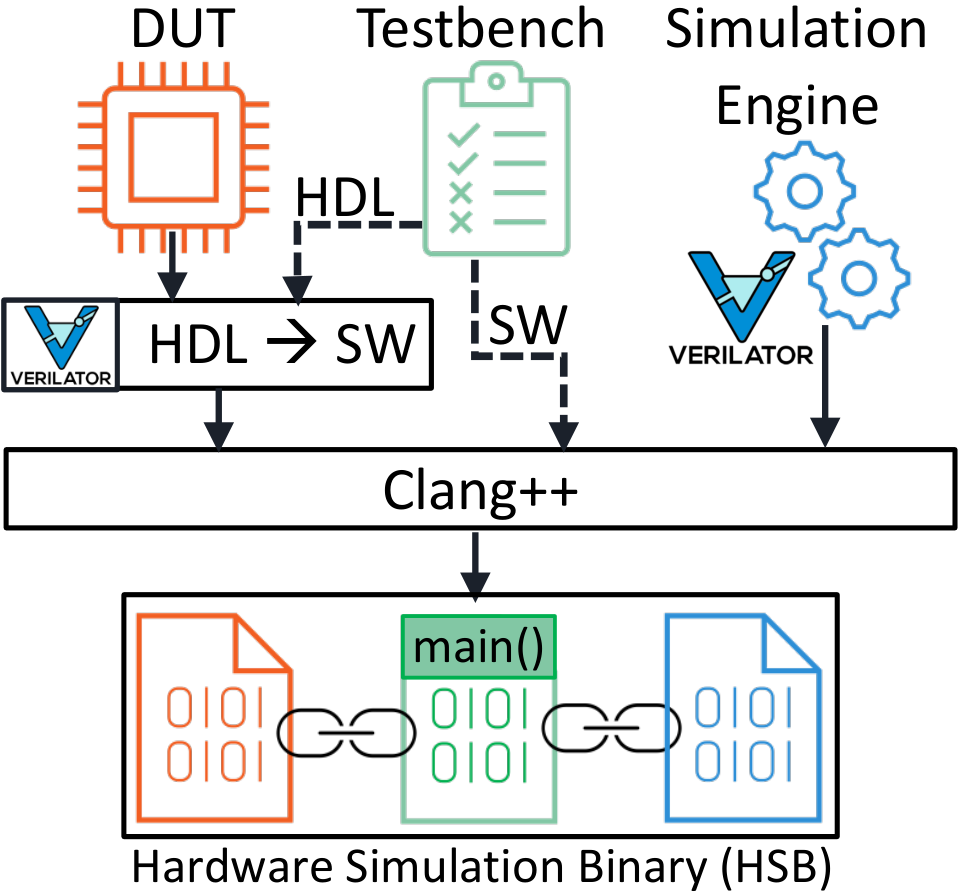
\includegraphics[width=0.4\textwidth]{hsb.png}
    \caption{
        برای اینکه یک سخت‌افزار شبیه‌سازی بشود باید ابتدا توصیف سخت‌افزار
        آن به یک مدل نرم‌افزاری مدل شده و در ادامه با
        \lr{testbench}
        و
        \lr{Simulation Engine}
        لینک شود.
        اجرای این فایل اجرایی با استفاده از یک سری از ورودی‌ها رفتار طراحی را شبیه‌سازی می‌کند.
    }
    \label{fig1}
\end{figure}
در ابتدا
\lr{HDL}
به یک مدل نرم‌افزاری برای مثال
\lr{C/C++}
تبدیل می‌شود سپس این مدل و
\lr{testbench}
با یک‌دیگر و یک موتور شبیه‌ساز لینک شده که با هم این یک
\lr{Hardware Simulation Binary (HSB)}
را شکل می‌دهند.
در آخر این
\lr{HSB}
با ورودی‌های که توسط
\lr{testbench}
تولید می‌شود اجرا شده و رفتار طراحی تحت آزمون بررسی می‌شود.
\subsubsection{ارزیابی تست}
بعد از اینکه عمل شبیه‌سازی انجام شد وضعیت سخت‌افزار تحت تست هم از درون و هم از خروجی‌ها
برای صحت بررسی می‌شود.
دو روش برای صحت‌سنجی وجود دارد
\begin{enumerate}
    \item بررسی ثابت
    \lr{Invariant Checking}
    \item مدل طلایی
    \lr{Golden Model}
\end{enumerate}
در بررسی ثابت یک مجموعه از
\lr{assertion}
ها برای بررسی موارد مربوط به طراحی استفاده می‌شود.
در
\lr{Model Checking}
یک مدل متفاوت از طراحی اصلی برای شبیه‌سازی رفتار صحیح طراحی تحت آزمون ساخته می‌شود
و خروجی‌ها به طراحی اصلی مقایسه می‌شود.
\subsection{فازور‌های نرم‌افزاری}
تست‌فاز نرم‌افزاری یک تست اتوماتیک شده است که هدف از انجام آن یافتن مشکلات امنیتی
در نرم‌افزار است. این روش به خاطر موفقیتی که در کشف مشکلات داشته است در صنعت
و جامعه متن‌باز از آن به شدت استفاده می‌شود.
به طور کلی تست فاز شامل سه مرحله است
\begin{enumerate}
    \item تولید تست
    \item مانیتور کردن اجرای تست
    \item بررسی خطا
\end{enumerate}
در زمان تولید تست یک ورودی برای برنامه ساخته می‌شود در مرحله بعدی این ورودی وارد برنامه می‌شود
و اجرای آن مانیتور می‌شود
در آخر اجرای اگر تست باعث ایجاد خطا در سیستم شد سیستم حالت را ذخیره می‌کند
و با استفاده از تستی که انجام داده شد بررسی آغاز می‌شود.
این پروسه تکرار می‌شود تا اینکه پوشش هدف تست به حد مورد نیاز برسد.
در این بخش سعی می‌شود که الگوریتم فازور معروف
\lr{AFL}
شرح داده شود.
در یک فازور نرم‌افزاری
نرم‌افزار تحت آزمون یا
\lr{Program Under Test (PUT)}
به صورت یک تابع خالص که یک آرایه‌از بایت‌ها را به عنوان ورودی می‌گیرد مدل می‌شود.
رفتار برنامه تحت تست فقط باید به ورودی وابسته باشد و برای همین هر ورودی
یک اجرای تست را توصیف می‌کند.
برای اینکه تضمین دهیم که نتایج تست قابل باز سازی است باید در هر بار اجرای تست
حالت داخلی برنامه را ریست کنیم. فازور‌های نرم‌افزاری از تصویر حافظه یا
\lr{Memory Snapshot}
برای این کار استفاده می‌کنند.
تا بعد از دادن ورودی برنامه را به حالت اولیه برگردانند.
هدف از مانیتور کردن در زمان تست این است که برای هر اجرا میزان کاورج سنجیده شود
و از این داده‌ها برای افزایش کاورج استفاده شود.
برای اینکه عمل بالا مؤثر باشد باید متریک کاورج مورد استفاده سبک باشد تا اجرای تست را
تحت تأثیر قرار ندهد.
و در این کنار به حدی دقیق باشد تا بتواند به
\lr{Fuzzing Engine}
برای پیدا کردن مسیر مؤثر کمک کند.
متریک کاورجی که توسط فازور
\lr{AFL}
استفاده می‌شود یک نسخه تقریبی از پوشش برنچ است.
در حین اجرای برنامه هر
\lr{Basic Block}
از برنامه یک شناسه منحصر به فرد رندوم می‌گیرد
وقتی برنامه اجرای خود را شروع کرد بین هر شاخه از برنامه که مبدا و مقصد دارد
این شناسه از مبدا با مقصد هش شده و در یک جدول قرار می‌گیرد
که به این صورت نشان می‌دهد که اجرای برنامه چند با از این مسیر عبور کرده است.
که سنجش این موضوع به این دلیل است که ممکن است دو بار رد شدن از یک مسیر برای ما جذاب باشد
ولی این کانتر تا مقادیر محدودی از گذر را نشان می‌دهد چون که بیشتر از یک مقدار خاص دیگر جذابیتی از نظر
بیشتر کردن کاورج ندارد.
در هسته این فازور یک
\lr{Fuzz Engine}
وجود دارد که ورودی‌های جدید را برای ما با استفاده از الگوریتم
~\ref{alg1}
انتخاب می‌کند
\lr{
    \begin{algorithm}
        \label{alg1}
        \caption{Compute some function by recursive algorithm}
        Given: program pm set of initial inputs i
        Returns: a set of generated test inputs
        \begin{algorithmic}[1]
            \State $S \gets I$
            \State $totalCoverage \gets 0$
            \Repeat
            \For{$inputs in S$}
            \For{$1 \le i \le NUMCANDIDATES(input)$}
            \State $candidate \gets MUTATE(input,S)$
            \State $coverage \gets RUN(p, candidate)$
            \If{$coverage \not\subset totalCoverage$}
            \State $S \gets S \cup \{ candidate \}$
            \State $totalCoverage \gets totalCoverage \cup coverage$
            \EndIf
            \EndFor
            \EndFor
            \State $asd$
            \Until{A}
            \State \textbf{return} S
        \end{algorithmic}
    \end{algorithm}
}
این الگوریتم با یک ست معین از ورودی‌ها شروع می‌کند در هر بار از اجرا یک ورودی انتخاب شده
و بر روی این ورودی یک سری تغییرات اعمال می‌شود که توسط برنامه اجرا می‌گردد.
اگر این اجرا به نقطه‌ی جدیدی از کاورج دست پیدا کند این ورودی به مجموعه
\lr{S}
اضافه می‌شود.
الگورتیم ایجاد تغییرات بر روی ورودی به دو نوع
\lr{Deterministic}
و
\lr{Non-Deterministic}
تقسیم بندی می‌شود.
یک
\lr{Mutator}
تابعی است که یک تست را تحویل می‌گیرد و بر روی آن یک سری تغییرات اعمال می‌کند تا تست‌های
دیگری را تولید کند.
یک مثال از الگورتیم‌های قطعی در
\lr{AFL}
الگورتیم
\lr{bitflip 1/1}
است که یک فرزند از تست‌کیس به ازای هر والد تولید می‌کند.
لیست الگوریتم های قطعی در جدول
\ref{tab1}
نشان داده شده‌اند
\begin{table}[htbp]
    \caption{Deterministic Mutations Techniques}
    \begin{center}
    \lr{
    \begin{tabular}{p{0.5\linewidth}l}
    Description & Name \\
    \hline
    flip single bit & bitflip 1/1 \\
    flip two adjacent bits & bitflip 2/1 \\
    flip four adjacent bits & bitflip 4/1 \\
    flip single byte & bitflip 8/8 \\
    flip two adjacent bytes & bitflip 16/8 \\
    flip four adjacent bytes & bitflip 32/8 \\
    treat single byte as 8-bit integer, add/sub values from 0 to 35 & arith 8/8 \\
    treat two adjacent bytes as 16-bit integer, add/sub values from 0 to 35 & arith 16/8 \\
    treat four adjacent bytes as 32-bit integer, add/sub values from 0 to 35 & arith 32/8 \\  
    \end{tabular}
    }
    \label{tab1}
    \end{center}
\end{table}
تغییرات غیر مشخص یا
\lr{Non-Deterministic}
در مرحله
\lr{havoc}
انجام می‌شوند.
در هر بار اجرای
\lr{havoc}
از ۲ تا ۱۲۸ تغییر رندوم بر روی ورودی والد انجام می‌شود.
که در جدول
\ref{tab2}
به آن‌ها پرداخته شده است
\begin{table}[htbp]
    \caption{Non-Deterministic havoc Mutations}
    \begin{center}
    \lr{
    \begin{tabular}{p{0.5\linewidth}l}
    Description & Name \\
    \hline
    flip a random bit & bitflip \\
    overwrite a random 8-bit integer with interesting value & interest 8 \\
    overwrite a random 16-bit integer with interesting value & interest 16 \\
    overwrite a random 32-bit integer with interesting value & interest 32 \\
    treat random single byte as 8-bit integer, add/sub one value from 0 to 35 & arith 8/8 \\
    treat two random adjacent byte as 16-bit integer, add/sub one value from 0 to 35 & arith 16/8 \\
    treat four random adjacent byte as 32-bit integer, add/sub one value from 0 to 35 & arith 32/8 \\
    overwrite random byte with random value & random 8 \\
    delete a random sequence of bytes & delete \\
    clone a random sequence of bytes & clone \\
    overwrite a random sequence of bytes & overwrite \\    
    \end{tabular}
    }
    \label{tab2}
    \end{center}
\end{table}
مهم‌ترین نقطه قوت روش
\lr{Coverage-Directed Mutational Fuzzing}
به روش‌های صحت‌سنجی فرمال این است که هزینه طراحی کردن آن پایین است و به راحتی می‌تواند
با سیستم‌های بزرگ اسکیل شود.
\section{
    رویکرد
    مقاله
    \lr{Hardware Fuzzing}
}
در این بخش به رویکرد مقاله
\cite{hf}
می‌پردازیم.
مقاله
\cite{hf}
از روند خود به عنوان
\lr{Hardware Fuzzing}
یاد می‌کند.
برای اینکه بتوانیم از پیشرفت‌های در زمینه فازور‌های نرم‌افزاری در سخت‌افزار استفاده کنیم باید بتوانیم
که طراحی‌های سخت‌افزاری را به نرم‌افزاری نگاشت کنیم.
سه بخش اساسی این روش عبارت‌اند از:
\begin{enumerate}
    \item نگاشت سخت‌افزار به فایل اجرایی نرم‌افزاری
    \item سنجش پوشش سخت‌افزاری در نرم‌افزار
    \item ترجمه تست‌کیس‌های تولید شده توسط فازور برای استفاده در طراحی تحت آزمون
\end{enumerate}
\subsubsection{نگاشت سخت‌افزار به نرم‌افزار}
برای نگاشت سخت‌افزار به نرم‌افزار در مقاله
\cite{hf}
از نرم‌افزار
\lr{Verilator}~\cite{ver}
استفاده شده است که این نرم‌افزار مدل‌های
\lr{HDL}
را به یک مدل
\lr{C++}
تبدیل می‌کند که مدل سخت‌افزاری را می‌تواند سیکل به سیکل شبیه‌سازی کند.
برای اینکه با این مدل ارتباط برقرار کنیم در یک حلقه باید تابع
\lr{\textit{eval()}}
را فراخوانی کنیم که هر بار فراخوانی این تابع مدل‌ را با ورودی‌هایی که به مدل داده‌ایم آپدیت می‌کند.
در دو بار فراخوانی تابع
\lr{\textit{eval()}}
مدل را یک کلاک سایکل جلو می‌برد.
\subsubsection{سنجش پوشش سخت‌افزار}
تکنیک‌های
\lr{CDG}
برای اینکه بتوانند فضای حالت طراحی را به خوبی پیمایش کنند باید از متریک پوشش اجرای قبلی استفاده کنند
تا بتوانند تست‌کیس بعدی را به خوبی تولید کنند.
دو متریک اصلی برای سنجش پوشش در سخت‌افزار استفاده می‌شود که اولی
\lr{Code Coverage}
و دومی
\lr{Functional Coverage}
است.
درشت‌ترین و معمول‌ترین متریک برای سنجش پوشش کد سیستم تعداد خط‌های کد نوشته شده است.
از سوی دیگر متریک
پوشش کاربردی برای بررسی ویژگی‌هایی از طراحی تحت آزمون استفاده می‌شود که موردنظر طراح هستند
که این متریک‌ها توسط
\lr{SystemVerilog Coverage Points/Groups}
تعیین می‌شوند.
صرف‌نظر از روشی که استفاده می‌شود نگاشت پوشش شبیه‌سازی نرم‌افزاری به سخت‌افزار
سخت و زمان‌بر است.
\cite{slow}
برای اینکه بتوانیم پوشش طراحی تست آزمون را به خوبی بسنجیم مقاله
~\cite{rf}
از متریک‌های پوشش شخصی‌سازی استفاده می‌کنند.
این روش‌ها نیاز دارند که دیزاین سخت‌افزار را به یک زبان میانی تبدیل کنند
و در این زبان میانی مانند
\lr{FIRRTL}
یک سری بهینه‌سازی‌های کامپایلری انجام دهند تا بتوانند این موارد را در کد سخت‌افزاری وارد کنند.
مقاله
\cite{hf}
به جای اینکه روش‌های فعلی
\lr{CDG}
را بهبود بخشد سعی می‌کند روش‌های نرم‌افزاری را به صورت مستقیم به دنیای سخت‌افزار بیاورد.
فازور‌های نرم‌افزاری از روش
\lr{edge coverage}
استفاده می‌کنند.
به دلیل اینکه
\lr{Verilator}
کد
\lr{C++}
مستقیم تولید می‌کند می‌توان نتیجه گرفت که اگر ما تولید تست را برای افزایش
پوشش در مدل نرم‌افزاری که از متریک لبه استفاده می‌کند، بهینه کنیم کاورج سخت‌‌افزار را نیز بهبود می‌بخشیم.
لازم به ذکر است که ترجمه کاورج از نرم‌افزار به سخت‌افزار توسط
lr{Verilator}
انجام می‌شود.
\subsubsection{تفسیر تست‌های تولید شده توسط فازور}
نرم‌افزارها توسط یک ورودی تمامی تغییر وضعیت‌های مورد نیاز خود را انجام می‌دهند
به صورتی که به ورودی این برنامه‌ها یک آرایه از بایت‌ها داده می شود که در صورت بروز خطا
می‌شود این آرایه از بایت‌ها را بررسی کرد.
ولی در سخت‌افزار یک دنباله از ورودی‌ها لازم است.
برای مثال برای یک قفل ۴ عددی
باید یک دنباله از ورودی‌ها را وارد کنیم.
برای همین در مقاله
\cite{hf}
روشی پیشنهاد داده شده‌است که بتواند ورودی‌های تک بعدی را به دو بعد زمان و مکان
نگاشت کند.
\section{رویکرد مقاله
\lr{RFuzz}
}
روش
\lr{Coverage-Guided Mutational Fuzz Testing}
بر پایه تولید ورودی بنا شده است که این تولید ورودی از پوشش انجام شده بازخورد می‌گیرد که این
روش به طور مستقیم نمی‌تواند به سخت‌افزار نگاشت شود.
یک سخت‌افزار مانند یک نرم‌افزار یک ورودی از بایت‌ها را دریافت نمی‌کند بلکه ورودی‌ها به صورت
سیم هستند که در هر سایکل می‌توانند مقدار متفاوتی داشته باشند.
علاوه‌ بر این روش‌های
\lr{Memory Snapshoting}
که در فازور‌های نرم‌افزاری برای برگرداندن وضعیت نرم‌افزار به حالت اولیه استفاده می‌شوند نمی‌توانند
به صورت مستقیم به
\lr{FPGA}
اعمال شوند.
همچنین پوشش بر پایه برنچ نیز نمی‌تواند به صورت مستقیم به کد
\lr{RTL}
نگاشت شود چون‌که برنچ در سخت‌افزار یک مالتی‌پلکسر است که در هر سایکل می‌تواند
ورودی متفاوتی داشته باشد.
در این بخش مقاله
\cite{rf}
به مشخص کردن روش انتخابی برای حل کردن مشکلاتی از این قبیل می‌پردازد
\subsubsection{تعریف ورودی‌ها}
در مدارات
\lr{RTL}
معمولا یک ماژول سطح بالا دارند که این ماژول سطح بالا به تولید‌کننده تست متصل شده.
در این روش تمامی پین‌های ورودی در کنار هم قرار می‌گیرند و یک بردار از بیت‌ها را تشکیل می‌دهند
که این بردار یک ورودی در یک سایکل را نشان می‌دهد که این به
فازور این اجازه را می‌دهد که روی یک آرایه‌ از بیت‌ها تغییرات خودش را انجام دهد.
\subsubsection{اجرای تست به صورت
\lr{Deterministic}
}
برای اینکه اجرای تست‌ها به صورت قطعی و قابل دوباره‌سازی انجام گیرد باید اجرای برنامه تحت تست فاز
از یک حالت مشخص شروع شود.
ریست کردن یک برنامه به یک حالت مشخص می‌تواند زمان زیادی را از ما بگیرد.
فازور‌های معروف مانند
\lr{AFL}
از فراخوانی سیستمی
\lr{fork}
برای این‌کار استفاده می‌کنند.
ریست کردن یک مدار
\lr{RTL}
که بر روی یک
\lr{FPGA}
پیاده‌سازی شده است چالش‌های خودش را دارد که نیاز است به آن‌ها پرداخته شود.
در مقاله
\cite{rf}
در مورد دو موضوعی که برطرف شده است در قسمت‌های آتی صحبت خواهد شد.
\subsubsection{\lr{Register Meta Reset}}
مدارات ریست در رجیستر‌ها می‌توانند جای زیادی را در ویفر به خود اختصاص دهند
به همین دلیل معمولا از طراحی‌ها حذف می‌شوند
برای همین مقدار آن‌ها در موقع ریست مدار نامشخص می‌باشد.
شبیه‌ساز‌های کلاسیک به طور معمول این مقدار را
\lr{X}
می‌نامند که نشان می‌دهد یک سیم مقدار نامشخصی دارد.
به دلیل این‌که این مقاله بر روی
\lr{FPGA}
شبیه‌سازی می‌شود نیاز است که از یک راه‌حل دو مقداره استفاده کنیم.
برای همین دو روش ارائه می‌شود که اول این است که مقدار اولیه رجیستر را به عوان قسمتی از ورودی
در نظر بگیریم و روش دوم این است که در هر بار از ریست یک مقدار از پیش تعیین شده را به رجیستر‌ها
بدهیم که در این مقاله از روش دوم استفاده شده است.
برای تحقق بخشیدن به این کار در توصیف میانی مدار در یکی از گذر‌های کامپایلری که بر روی
توصیف میانی یا 
\lr{IR}
کار می‌کند یک سیم
\lr{Meta Reset}
به مدار اضافه می‌شود.
که در ابتدای اجرای هر تست این لاین به مدت یک سایکل فعال شده تا مقدار اولیه مشخص شده
را در رجیستر قرار دهد.
\subsubsection{\lr{Sparse Memories}}
مموری به ندرت در مدارات موقع روشن شدن ریست می‌شود.
می‌توانیم برای بهینه‌تر کردن موضوع به جای اینکه کل حافظه را ریست کنیم فقط کلماتی از حافظه را
ریست کنیم که در در تست قبلی بر روی آن‌ها کار انجام شده است.
این روش برای هر پورت نوشتن حافظه نیاز به یک بافر دارد تا بتواند موارد نوشته شده را در خود نگه دارد
تا بعد از انجام تست بتواند به حالت قبل از تست برگردد.
به خاطر اینکه تست‌ها کوچک هستند می‌توان ایده دیگری برای حافظه قابل ریست تعبیه کرد.
برای این کار یک مموری پراکنده به این صورت تعبیه می‌شود که درصورتی عمل خواندن انجام شد
آخرین مقدار نوشته شده را برگردان و در صورتی که در آن آدرس نوشتنی انجام نشده بود مقدار صفر
را برگردان.
با استفاده از روش‌های
\lr{MetaReset}
و
\lr{SparseMem}
می‌توان عملیات ریست کردن طراحی تحت آزمون را در دو کلاک سایکل انجام داد.
\subsubsection{تعریف پوشش}
تعریف پوشش برای دو هدف سنجش کار نهایی و دادن فیدبک به فازور موردنیاز است.
بیشتر متریک‌های کاورج بر روی زبان‌های توصیف سخت‌افزار مانند
\lr{Verilog}
فعالیت می‌کنند.
سیستمی که توسط این مقاله پیشنهاد شده بر روی تمامی مقالات
\lr{RTL}
کار می‌کند پس باید متریک کاورج به صورت قابل سنتز تعریف شود.
در این مقاله به متریک
\lr{Mux Control Coverage}
توجه می‌شود که هر مالتی‌پلکسر دو به یک را به عنوان یک نقطه پوشش در نظر می‌گیرد.
مالتی‌پلکسر‌هایی با بیشتر از دو ورودی‌هم می‌توانند به یک سری از مالتی پلکسر‌های دو به یک تبدیل شوند.
این متریک برای این در نظر گرفته شده‌است که بتواند بر هر مدار توصیف سخت‌افزاری اجرا شود.
برای اینکه هر نقطه به طور کامل کاور شود به این نیاز داریم که در هر تست
هر دو مقدار
\lr{true}
و
\lr{false}
را به خود بگیرد.
در
\lr{FPGA}
این روش به کمترین سخت‌افزار ممکن نیاز دارد به طوری که با دو مالتی‌پلکسر یک بیتی و دو رجیستر
یک بیتی می‌توان این روش را پیاده‌سازی کرد.
\subsubsection{الگوریتم‌های تغییر ورودی}
ورودی‌ که توسط این مقاله تعریف شده است به ما اجازه می‌دهد که الگوریتم‌های
\lr{AFL}
را به طور مستقیم پیاده‌سازی کنیم.
در ابتدا از الگوریتم‌های قطعی برای تولید ورودی استفاده می‌شود
بعد از اینکه ورودی‌های قطعی تمام شدند به سراغ ورودی‌های غیر قطعی می‌رویم.
برای هر تغییری که سایز ورودی‌ انجام می‌شود و این سایز بیشتر از تعداد سیم‌های طراحی باشد
برای این مقادیر صفر قرار می‌دهیم.
\subsubsection{قیود رابط}
در تست سخت‌افزار پیش‌فرض‌هایی وجود دارد که توسط
\lr{Stimuli Generator}
رعایت می‌شوند.
یک مثال برای این موضوع این است که یک باس حافظه می‌تواند به این موضوع اتکا
کند که شرکت‌کنندگان به پروتکل احترام می‌گذارند.
یک راه‌‌حل برای حل کردن این موضوع این است که یک آداپتور برای طراحی وجود داشته باشد
که ورودی‌های بدون قید را از فازور دریافت کرده و از روی آن‌ها ورودی با قید بسازد.
اینکه ما از هر ورودی بازخورد دریافت می‌کنیم می‌تواند کار را راحت‌تر کند.
می‌توان یک مانیتور تعبیه کرد که این مانیتور ورودی‌های بی‌اعتبار را تشخیص دهد.
که این مانیتور قابل سنتز یک خروجی
\lr{Valid}
به ما می‌دهد که به عنوان بازخورد به فازور می‌دهیم
در ابزار تولید شده در این مقاله دو نقشه پوشش نگهداری می‌شود که یکی مربوط به پوشش
ایجاد شده توسط ورودی‌های غیرمعتبر است و دیگری مخصوص ورودی‌های معتبر است
\section{پیاده‌سازی مقاله
\lr{Hardware Fuzzing}
}
ابزار
\lr{Verilator}
و کامپایلر‌هایی که فایل اجرایی را برای اجرا توسط فازور آماده می‌کنند برای دو موضوع
ترجمه سخت‌افزار به نرم‌افزار و ترجمه پوشش راه‌کار‌هایی را ارائه می‌دهند.
ولی در مورد تفسیر تست‌های تولید شده به ما راه‌حل مناسبی ارائه نمی‌دهند.
برای همین در این بخش در مورد ساخت تست‌بنچ و تفسیر آن توضیحاتی داده می‌شود.
\subsubsection{تولید‌کننده تست عمومی}
برای اینکه فازور‌های نرم‌افزاری را با سخت‌افزار هماهنگ کنیم نیاز است که یک تولید‌کننده تست عمومی
داشته باشیم که ورودی‌های یک بعدی را به یک دنباله از ورودی‌های دو بعدی تبدیل می‌کند.
تولید‌کننده تست این مقاله بایت‌های تولید شده توسط فازور را می‌خواند و آن‌ها را به پورت‌های
سخت‌افزار نگاشت می‌کند و یک سایکل دیزاین را جلو می‌برد و  این کار را آنقدر ادامه می‌دهد
تا بایتی برای عملیات وجود نداشته باشد.
رابطی چند بعدی که ورودی‌های فازور را به چند بعد زمان و مکان نگاشت می‌کرد
به طراحی وابسته است و نمی‌تواند بر روی تمامی طراحی‌ها فعالیت کند.
برای همین یک مهندس درستی‌سنجی باید تولید‌کننده تست را برای هر طراحی هماهنگ کند.
برای اینکه این مشکل حل شود از روشی که مهندسین سخت‌افزار برای متصل کردن هسته‌های
\lr{IP}
\cite{opentitan}
استفاده می‌کنند استفاده شده است.
برای همین برای انجام تست فاز بر روی هسته‌های
\lr{IP}
از رابط باس آن‌ها استفاده می‌کنیم.
تولید‌کننده تست فعلی که برپایه باس کار می‌کند بر اساس
\lr{TileLink Uncached Lightweight (TL-UL)}
ساخته شده‌است.
\cite{tilelink}
\subsubsection{انجام تست‌فاز در اسکیل بزرگ}
تست‌فاز منابع زیادی از سیستم می‌برد و منطقی نیست که بر روی یک نود انجام شود
برای همین این مقاله یک
\lr{Hardware Fuzzing Pipeline (HWFP)}
را معرفی کرده است که از مرحال زیر را انجام می‌دهد که برای این‌کار از کلاد گوگل استفاده می‌کند
\begin{enumerate}
    \item ترجمه طراحی از زبان توصیف سخت‌افزار به نرم‌افزار با استفاده از
    \lr{Verilator}
    \item کامپایل و لینک کردن آن با تولید‌کننده تست
    \item اجرای آن برای مدتی از زمان
    \item سنجش پوشش و ترجمه پوشش از نرم‌افزار به سخت‌افزار
    \item سیو کردن داده‌های پوشش و تست‌ها در صورت وجود خطا
    \item خاموش کردن ماشین مجازی
\end{enumerate}
این روش فقط از ابزار متن‌باز استفاده می‌کند که به مهندسین درستی‌سنجی کمک می‌کند
تا هزینه‌های خود را کمتر کنند.
\section{پیاده‌سازی مقاله
\lr{RFuzz}
}
متودی‌ که در مقاله
\cite{rf}
معرفی شده است در نرم‌افزار متن‌باز
\lr{RFuzz}
پیاده‌سازی شده‌است.
بخش اول این‌ نرم‌افزار قسمت تولید تست و راه‌بری تست است که بر روی یک توصیف سخت‌افزار
به نام
\lr{FIRRTL}
پیاده‌سازی شده است
\cite{firrtl}.
این ابزار به صورت اتوماتیک برای شبیه‌سازی‌های بر پایه
\lr{FPGA}
و نرم‌افزار تست تولید می‌کند.
این ابزار به زبان توصیف سخت‌افزار وابستگی ندارد مادامی که
این زبان بتواند به زبان میانی
\lr{FIRRTL}
ترجمه شود.
\subsubsection{راه‌بری}
تبدیل‌های سفارشی به عنوان پاس‌های کامپایلر که بر روی کامپایلر
\lr{FIRRTL}
پیاده‌سازی شده‌اند که این کامپایلر کمک می‌کند
تا کد‌های بلااستفاده را نیز از طراحی حذف کند تا سایز کاورج مورد‌نیاز
کم بماند.
تکنیک
\lr{MuxCov}
به صورت اتوماتیک سیم‌های کاورج را با پیمایش توصیف مدار می‌سازد.
\subsubsection{تولید تست}
با دادن اطلاعات طراحی بخش تولید تست برای هر طراحی
\lr{RTL}
یک بخش تولید تست می‌سازد.
این بخش طراحی تحت آزمون را
\lr{instantiate}
می‌کند و پین‌های کاورج را متصل می‌کند.
تولید‌کننده تست توسط کامپایلر
\lr{FIRRTL}
بهینه شده تا بتواند ورودی‌های مؤثر را تولید کند.
همچنین این ابزار برای
\lr{FPGA}
یک بافر می‌سازد تا ارتباط با فازور سریع‌تر انجام شود.
در آخر سیستم‌ تولید تست اطلاعاتی را مخصوص طراحی تحت تست تولید می‌کند
که این اطلاعات شامل شمارنده‌های کاورج و ورودی‌ها و فرمت بافر‌ها هستند.
فازور از این اطلاعات برای تولید تست استفاده می‌کند.
\subsubsection{فازور}
طراحی تحت آزمون و شمارنده‌های کاورج می‌توانند روی
\lr{FPGA}
ستتز شوند و در این کنار تولید ورودی و آنالیز کاورج توسط فازور
بر روی یک پردازنده سریع انجام می‌شود.
اجرای فازور بر روی پردازنده عمومی به ما اجازه می‌دهد تا ورودی‌های
منعطفی را برای سیستم تولید کنیم و استراتژی‌های بازخورد
قوی‌تری را تولید کنیم.
شکل
~/ref{fig3}
نشان می‌دهد که این فازور چگونه با سیستم ارتباط دارد.
\begin{figure}[!t]
    \centering
    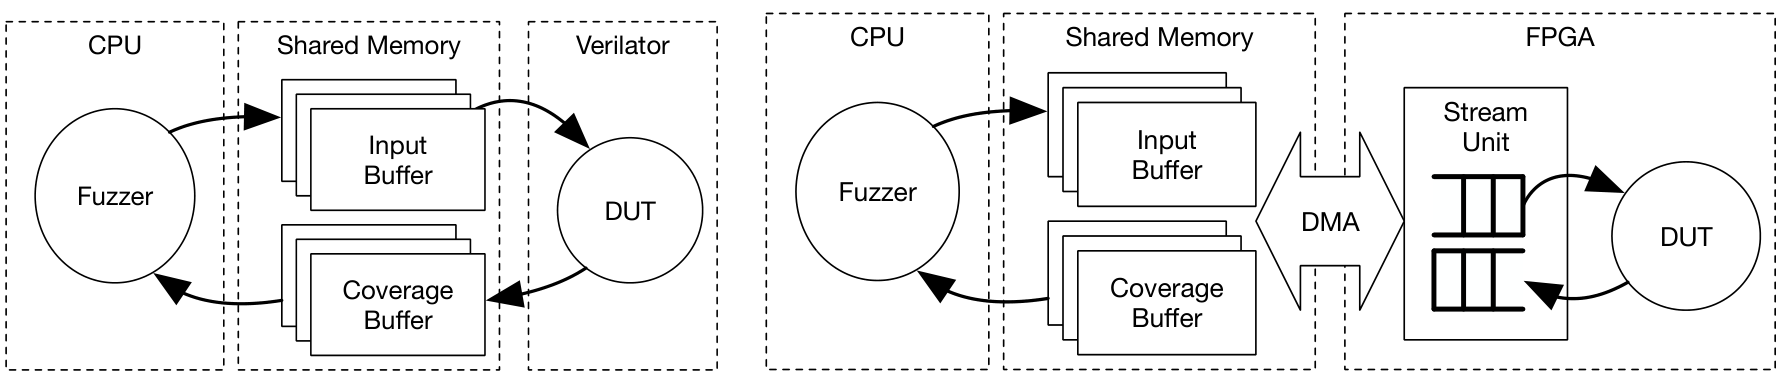
\includegraphics[width=0.5\textwidth]{rfuzz.png}
    \caption{
        توصیف روش ارتباطی فازور با سیستم و طراحی
    }
    \label{fig3}
\end{figure}

\section{نتایج}
مقاله
\cite{hf}
در ابتدا یک مقایسه با مقاله
\cite{rf}
انجام می‌دهد که به شرح زیر است.
برخلاف روش مقاله
،
مقاله
\lr{RFuzz}
سخت‌افزار سنجش کاورج را در توصیف سخت‌افزار قرار می‌دهد
و همینطور مقاله
\lr{RFuzz}
هیچ تست‌ فازی را بر روی باس عمومی استاندارد‌سازی نکرده است.
برای اینکه مقایسه انجام شود روند دو مقاله با یکدیگر مقایسه شده است
و برای این مقایسه از سنجش تعداد خط کد کاور شده استفاده شده است.
در شکل
~\ref{fig3}
این مقایسه بعد از ۲۴ ساعت نشان‌داده شده است
نتایج نشان می‌دهند که مقاله
\lr{Hardware Fuzzing}
حدود ۲۶.۷۰ درصد از
\lr{RFuzz}
در زمینه کاورج بهتر  عمل کرده است.
\begin{figure}[!t]
    \centering
    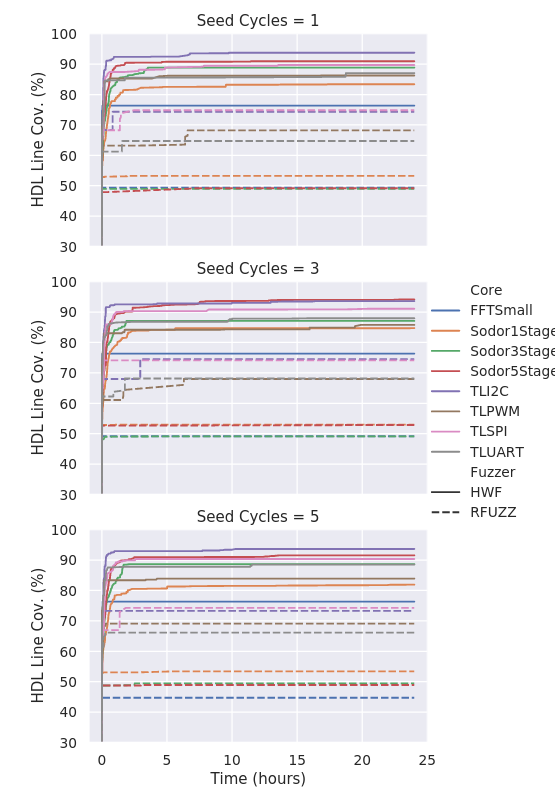
\includegraphics[width=0.5\textwidth]{res1.png}
    \caption{
    تست فاز هشت طراحی متفاوت توسط روش‌های پیشنهادی بررسی شده    
    }
    \label{fig3}
\end{figure}
\subsection{نتایج مقاله
\lr{Hardware Fuzzing}
}
در این بخش یکی از
\lr{IP}
های
\lr{OpenTitan}
بررسی می شود که در این بخش
هسته‌های زیادی مانند
\lr{AES}
،
\lr{HMAC}
، و
\lr{RISC-V}
بررسی شده‌اند.
این ‌هسته‌ها همه توسط پروتکل باس
\lr{TL-UL}
کنترل می‌شوند.
با استفاده از یک
\lr{Seed}
خالی نتایج شکل
~\ref{fig4}
تولید شده است.
\begin{figure}[!t]
    \centering
    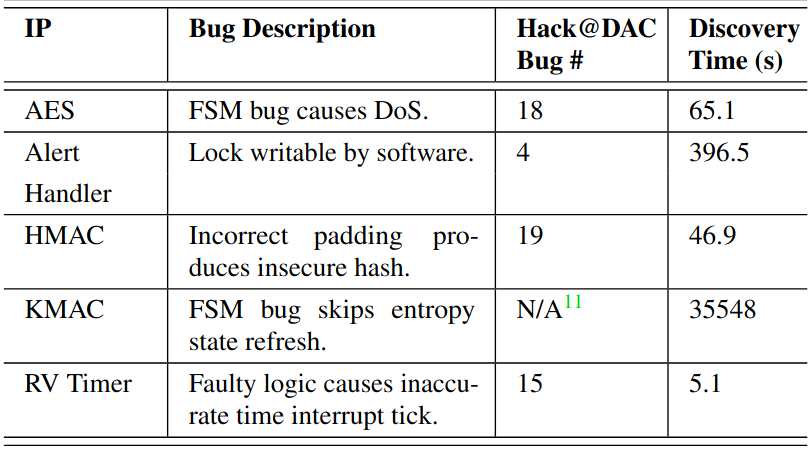
\includegraphics[width=0.5\textwidth]{res3.png}
    \caption{
        تست فاز پنج
        \lr{IP}
        معرفی شده توسط پروژه
        \lr{OpenTitan} 
    }
    \label{fig4}
\end{figure}
با وجود اینکه پوشش متریک مهمی است هدف اصلی پیدا کردن مشکل در
طراحی تحت آزمون است.
برای این‌کار چهار باگ مشابه که در مسابقه
\lr{Hack@DAC}
استفاده شده بود در طراحی‌ها قرار گرفت
در جدول
~\ref{fig5}
زمانی که سیستم صرف کرد تا به باگ برسد را نشان می‌دهد
\begin{figure}[!t]
    \centering
    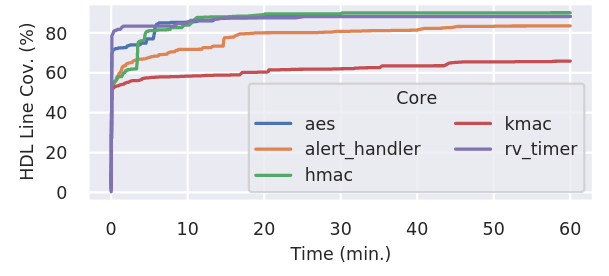
\includegraphics[width=0.5\textwidth]{res2.png}
    \caption{
        زمان کشف باگ توسط فازور
    }
    \label{fig5}
\end{figure}
\subsection{نتایج مقاله
\lr{RFuzz}
}
در نتایج مقاله
\lr{RFuzz}
پنج دیزاین سخت‌افزاری بررسی شده است.
\begin{enumerate}
    \item باس
    \lr{Tile Link}
    \item \lr{FFT}
    \item \lr{RISC-V Sodor Cores}
    \item \lr{RISC-V Rocket Core}
\end{enumerate}
برای سنجش این مقاله از
شبیه‌سازی نرم‌افزاری بر روی کلاد آمازون استفاده می‌کند.
هر تست فاز بر روی هسته مخصوص به خودش انجام می‌شود و هر آزمون در این
سیستم چهار بار با
\lr{Seed}
های متفاوت انجام می‌شود و نتایج میانگین گیری می‌گردد. \\
حین‌ انجام هر تست نتایج هر ست از تست‌ها در دیسک نوشته می‌شود.
برای اینکه نتایج سنجیده شوند از یک سری اسکریپت پایتون استفاده شده است تا
نتایج کاورج را محاسبه کنند.
به خاطر اینکه سرعت در این تست برای ما مهم نیست می‌توانیم هر بار
نرم‌افزار شبیه‌ساز را ریستارت کنیم تا مطمئن باشیم نتایج هر تست
از هم مستقل هستند.
ممکن است بعضی از ماکس‌ها نتوانند توسط ورودی‌های فازور کنترل شوند
برای همین هیچ تضمینی نیست که کاورج به ۱۰۰ درصد برسد.
\begin{figure}[!t]
    \centering
    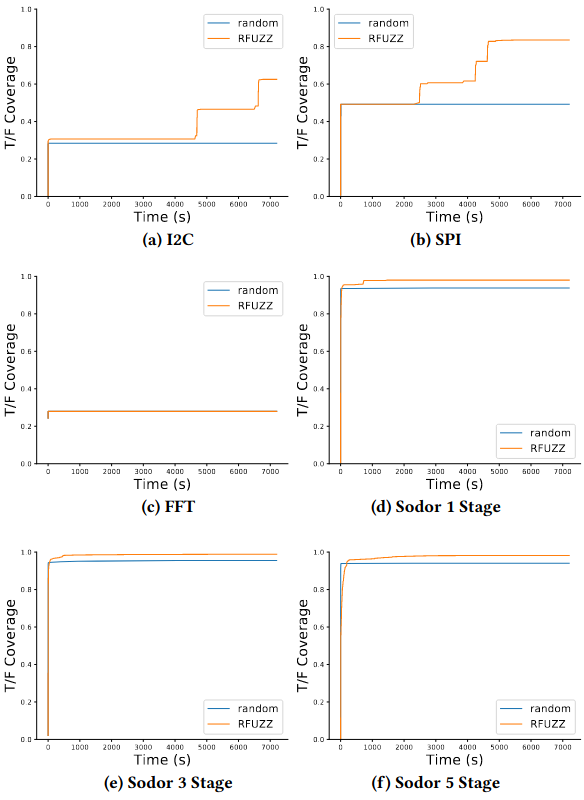
\includegraphics[width=0.4\textwidth]{res4.png}
    \caption{
        نتایج فازور
        \lr{RFuzz}
    }
    \label{fig5}
\end{figure}
\section{نتیجه}
بررسی این مقالات به ما نشان داد که روش‌های تست فاز که زیر مجموعه
روش‌های
\lr{CDG}
هستند ویژگی‌های خیلی مثبتی دارند. \\
استفاده از پیشرفت‌های انجام شده در حوزه فازور‌های نرم‌افزاری می‌تواند به ما کمک کند
تا بتوانیم کاورج در سیستم‌های سخت‌افزاری را بالا ببریم. \\
مقاله اول سعی می‌کند تا بتواند فازور‌های نرم‌افزاری را به صورت مستقیم وارد سخت‌افزار کند. که
در این موضوع تا موفق بوده و باعث شده است که استفاده از تکنیک‌های
\lr{CDG}
برای مهندسین درستی‌سنجی ساده‌تر بشود.
ولی در این کنار استفاده از این فازور به صورت تنها بسیار دشوار می‌باشد
و نگاشت کاورج از نرم‌افزار به سخت‌افزار بسیار طولانی می‌باشد.
مورد مثبتی که این روش به ما ارائه داد این است که این سیستم به گونه‌ای طراحی شده است که می‌تواند
در کلاد‌های دردسترس اجرا شود و به این گونه هزینه اجرای این سیستم برای مهندسین درستی‌سنجی
و شرکت‌های مربوطه کم خواهد بود. \\
روش‌
\lr{RFuzz}
برای استفاده از تکنیک‌هایی که در فازور معروف
\lr{AFL}
معرفی شده است، ساخته شده است.
ویژگی اصلی این فازور این است که می‌تواند برای سرعت بخشیدن به تست از
\lr{FPGA}
استفاده کند که این روش به دلیل استفاده از شتاب‌دهنده
بدون استفاده از کلاد نیز می‌تواند راه‌اندازی شود و همچنین می‌تواند از امولاتور‌‌های
صنعتی موجود نیز بهره ببرد که این موضوع برای درستی‌سنجی در زمانی
که کلاد یا کلاستر‌های کامپیوتری برای شبیه‌سازی نرم‌افزاری در دسترس نیستند
مؤثر می‌باشد.
به طور کلی در کار‌های آتی می‌توان به این موضوع که چگونه نگاشت
کاورج را سریع‌تر کرد و همچنین روش‌هایی برای فازور تعبیه شود
که ما را از باس‌های استاندارد بی‌نیاز کند پرداخت.
\section*{References}

\begin{thebibliography}{00}
\bibitem{hf} \lr{Trippel, T., Shin, K. G., Chernyakhovsky, A., Kelly, G., Rizzo, D., \& Hicks, M. (2022). Fuzzing hardware like software. In 31st USENIX Security Symposium (USENIX Security 22) (pp. 3237-3254).}
\bibitem{rf} \lr{Laeufer, K., Koenig, J., Kim, D., Bachrach, J., \& Sen, K. (2018, November). RFUZZ: Coverage-directed fuzz testing of RTL on FPGAs. In 2018 IEEE/ACM International Conference on Computer-Aided Design (ICCAD) (pp. 1-8). ACM.}
\bibitem{b1} \lr{Sophia Shao and Emma Wang. Die photo analysis. http://vlsiar
ch.eecs.harvard.edu/research/accelerators/die-photo-an
alysis/.}
\bibitem{b2} \lr{MITRE Corporation. Cve details: Intel: Vulnerability statistics, August
2019. https://www.cvedetails.com/vendor/238/Intel.html.}
\bibitem{b3} \lr{Kevin Laeufer, Jack Koenig, Donggyu Kim, Jonathan Bachrach, and
Koushik Sen. RFUZZ: coverage-directed fuzz testing of RTL on FPGAs. In IEEE/ACM International Conference on Computer-Aided
Design (ICCAD). IEEE, 2018.}
\bibitem{ver} \lr{Wilson Snyder. verilator. https://www.veripool.org/wiki/verilator.}
\bibitem{slow} \lr{Jing-Yang Jou and Chien-Nan Jimmy Liu. Coverage analysis tech-
niques for hdl design validation. Proceedings of Asia Pacific Chip
Design Languages, 1999}
\bibitem{opentitan} \lr{lowRISC Contributors. OpenTitan: Comportability Definition and
Specification, November 2020. https://docs.opentitan.org/doc/rm/comportability\_specification}
\bibitem{tilelink} \lr{SiFive Inc. SiFive: TileLink Specification, November 2020. Version 1.8.0.}
\bibitem{firrtl} \lr{Adam Izraelevitz, Jack Koenig, Patrick Li, Richard Lin, Angie Wang, Albert Mag-
yar, Donggyu Kim, Colin Schmidt, Chick Markley, Jim Lawson, and Jonathan
Bachrach. 2017. Reusability is FIRRTL Ground: Hardware Construction Lan-
guages, Compiler Frameworks, and Transformations. In ICCAD ’17}
\end{thebibliography}

\end{document}
